\documentclass{beamer}

\usepackage{graphicx}
\usepackage[utf8]{inputenc}

\title{GCM; The illegal attack}
\author{Mathias Hall-Andersen (rot256)}
\institute{Pwnies @ Copenhagen University}
\date{2017}

\begin{document}

\frame{\titlepage}

\begin{frame}
\frametitle{Mode of operation}
\begin{center}
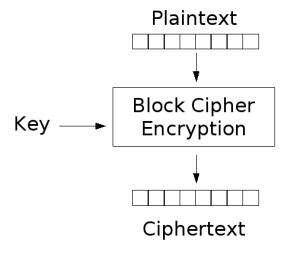
\includegraphics[height=0.5\textheight]{block_cipher.png}
\end{center}
\end{frame}

\begin{frame}
\frametitle{Mode of operation}
\begin{center}
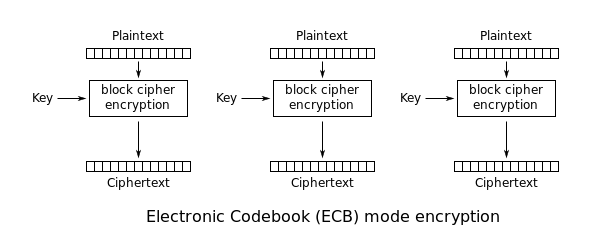
\includegraphics[width=\textwidth]{mode-ecb.png}
\end{center}
\end{frame}

\begin{frame}
\frametitle{Mode of operation}
\begin{center}
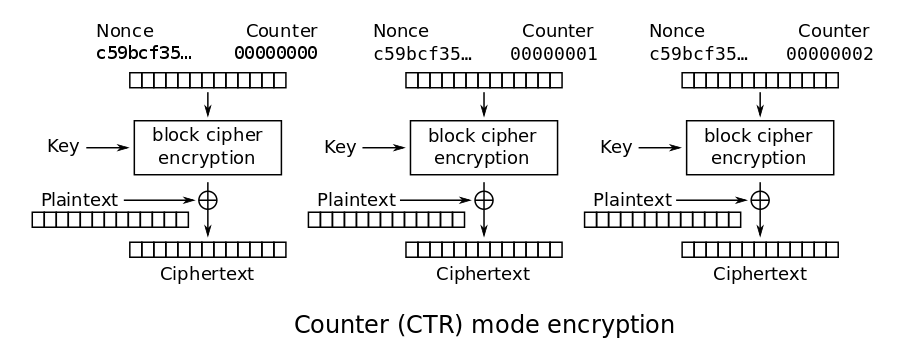
\includegraphics[width=\textwidth]{mode-ctr.png}
\end{center}
\end{frame}

\begin{frame}
\frametitle{Authenticated encryption}
\begin{center}
Encryption $\neq$ Authentication
\end{center}
\end{frame}

\begin{frame}
\frametitle{Galois Counter Mode (motivation)}
\begin{center}
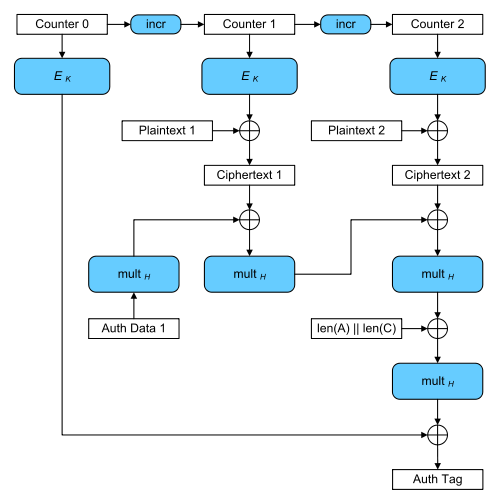
\includegraphics[height=0.7\textheight]{mode-gcm.png}
\end{center}
\end{frame}

\begin{frame}
\frametitle{Galois Counter Mode (motivation)}
\begin{center}
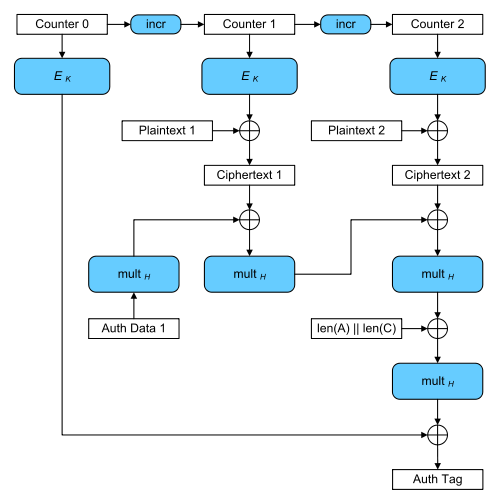
\includegraphics[height=0.7\textheight]{mode-gcm.png}
\end{center}
So what is $mult_{H}(\cdot)$?
\end{frame}

\begin{frame}
\frametitle{Some algebra}
\begin{center}
$mult_{H}(\cdot)$ is multiplication by $H$, \\
but not quite the way you might think...
\end{center}
\end{frame}

\begin{frame}
\frametitle{Rings}
\[
    (E, \cdot, +)
\]
St.
\[
    e_{1} \cdot (e_{2} + e_{3})
    =
    e_{1} \cdot e_{2}
    +
    e_{1} \cdot e_{3}
\]
\[
    \forall e_{1} :
    \exists e_{2} :
    e_{1} + e_{2} = 0
\]
Examples:
\[
    \mathbb{Z}
\]
\end{frame}

\begin{frame}
\frametitle{Fields}
Ring.
\[
    (E, \cdot, +)
\]
St.
\[
    \mathbb{Q}, \mathbb{R}
\]
\end{frame}

\begin{frame}
\frametitle{Rings \& Fields}
We will primarily be dealing with the field of two elements:
$1, 0$ \\
Where:
\begin{align}
    1 \cdot x &= x \text{ : 1 is the multiplicative identity} \\
    0 + x     &= x \text{ : 0 is the additive identity} \\
    1 + 1     &= 0 \text{ : the field has characteristic 2}
\end{align}
No magic.
Question:
If considered like bits, what common operations does
addition and multiplication in the field correspond to?
What implication does it have for bit-slicing techniques?
\end{frame}

\begin{frame}
\frametitle{Polynomials over Rings}
\end{frame}

\begin{frame}
\frametitle{Multiplication of polynomials over GF(2)}
\end{frame}

\begin{frame}
\frametitle{Additional resources}
So $mult_{H}(\cdot) : GF(2^{128}) \to GF(2^{128})$ \\
\vspace{3mm}
\textbf{Courses}
\begin{itemize}
    \item Algebra 1 @ Department of Mathematical Sciences (UCPH)
    \item Algebra 2 @ Department of Mathematical Sciences (UCPH)
    \item Computational Discrete Math @ DTU
\end{itemize}
\textbf{Books}
\begin{itemize}
    \item Algebra (2nd Edition) : Micheal Artin
    \item Abstract Algebra : Dummit \& Foote
\end{itemize}
\end{frame}

\begin{frame}
\frametitle{Galois Counter Mode (MAC calculation)}
\end{frame}

\begin{frame}
\frametitle{SageMath}
`SageMath is a free open-source mathematics software system licensed under the GPL.
 It builds on top of many existing open-source packages:
 NumPy, SciPy, matplotlib, Sympy, Maxima, GAP, FLINT, R and many more'
 - \url{https://www.sagemath.org/}
\end{frame}

\begin{frame}
\frametitle{SageMath}
sage or go to \url{https://cocalc.com/app}
\end{frame}


\begin{frame}
\frametitle{Nonce reuse attack}
Theorists care about proofs. \\
Pragmatists care about assumptions.
\end{frame}

\begin{frame}
\frametitle{Work session}
\end{frame}

\begin{frame}
\frametitle{Truncated nonce attack}
\end{frame}

\end{document}
